\section{Algorithms and backends}
\label{sec:architecture}

The codec separates \emph{what} is computed from \emph{how} it is executed
(Figure~\ref{fig:architecture}). Every numerically heavy step is a kernel written once, in
generic Rust, over a vector type \code{V}. The kernels know the algorithm (the operation order
of a transform schedule, the dequantization formula, the run-length scan of the tokenizer) but
nothing about instruction sets. A \emph{backend} is an implementation of the trait \code{Vf32}:
about twenty primitive operations on a vector of float32 lanes (Table~\ref{tab:primitives}).
Adding an instruction set means implementing those primitives, not rewriting the codec.

\begin{figure}[ht]
  \centering
  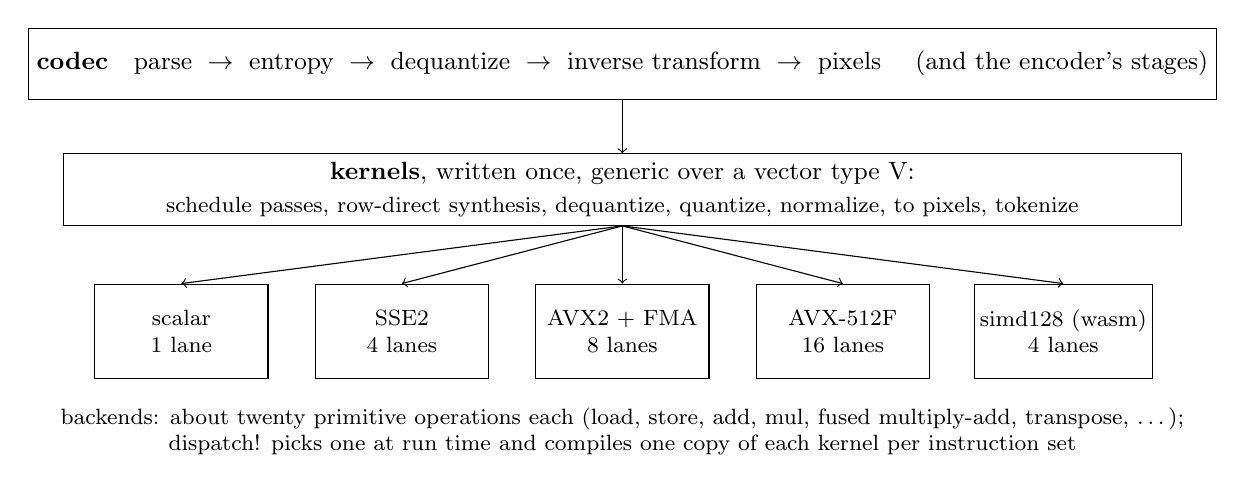
\begin{tikzpicture}[font=\small,
    layer/.style={draw,minimum height=9mm,align=center,inner sep=3pt},
    be/.style={draw,minimum height=12mm,minimum width=22mm,align=center,inner sep=2pt,font=\footnotesize}]
  % codec stages
  \node[layer,minimum width=14.2cm] (codec) at (0,3.2)
    {\textbf{codec}\quad parse \;$\to$\; entropy \;$\to$\; dequantize \;$\to$\; inverse transform \;$\to$\; pixels
     \quad(and the encoder's stages)};
  % kernels
  \node[layer,minimum width=14.2cm] (kern) at (0,1.6)
    {\textbf{kernels}, written once, generic over a vector type \code{V}:\\[1pt]
     \footnotesize schedule passes, row-direct synthesis, dequantize, quantize, normalize, to pixels, tokenize};
  % backends
  \node[be] (s) at (-5.6,-0.2) {scalar\\1 lane};
  \node[be] (sse) at (-2.8,-0.2) {SSE2\\4 lanes};
  \node[be] (avx) at (0,-0.2) {AVX2 + FMA\\8 lanes};
  \node[be] (avx5) at (2.8,-0.2) {AVX-512F\\16 lanes};
  \node[be] (w) at (5.6,-0.2) {simd128 (wasm)\\4 lanes};
  \node[font=\footnotesize,align=center,anchor=north] at (0,-1.05)
    {backends: about twenty primitive operations each (load, store, add, mul, fused multiply-add, transpose, \dots);\\
     \code{dispatch!} picks one at run time and compiles one copy of each kernel per instruction set};
  \draw[->] (codec) -- (kern);
  \foreach \b in {s,sse,avx,avx5,w} \draw[->] (kern.south) -- (\b.north);
\end{tikzpicture}

  \caption{Algorithms and backends. The codec calls kernels; the kernels are generic over the
  vector type; one implementation of the vector type exists per instruction set.}
  \label{fig:architecture}
\end{figure}

\begin{table}[ht]
  \centering\small
  \begin{tabular}{@{}lp{10.3cm}@{}}
    \toprule
    primitive & use \\
    \midrule
    \code{load}, \code{store}, \code{splat} & moving data; broadcasting a coefficient \\
    \code{add}, \code{sub}, \code{mul}, \code{div} & IEEE float32 arithmetic, identical on every backend \\
    \code{fmadd} & $a b + c$, fused where the hardware has FMA (fast mode only) \\
    \code{transpose} & a LANES$\times$LANES block (row passes of the analysis) \\
    \code{interleave} & merges even and odd outputs (row-direct synthesis) \\
    \code{min}, \code{max}, \code{trunc}, \code{select\_gt} & clamping, quantization \\
    \code{copysign}, \code{where\_nonzero} & dequantization without branches \\
    \code{from\_u8}, \code{store\_u8} & pixel conversion in and out \\
    \code{nonzero\_bits} & skipping zeros eight or sixteen at a time in the tokenizer \\
    \bottomrule
  \end{tabular}
  \caption{The vector interface. Each backend implements these operations with its intrinsics:
  \code{\_mm\_*} (SSE2), \code{\_mm256\_*} (AVX2 and FMA), \code{\_mm512\_*} (AVX-512F) or
  \code{f32x4\_*} (WebAssembly SIMD); the scalar backend uses plain Rust.}
  \label{tab:primitives}
\end{table}

\subsection{Dispatch}

Only inside a function that carries the attribute \code{\#[target\_feature]} does Rust
compile code for a given instruction set. A macro, \code{dispatch!}, turns each generic entry point into one
such wrapper per backend and selects one at run time from the CPU's features
(Algorithm~\ref{alg:dispatch}). The generic code is inlined into each wrapper, so the
intrinsics of the backend are inlined too, with no call per operation. One subtlety cost a
factor of ten during development: closures do not inherit target features, so a kernel called
from inside a thread's closure ran with every vector operation as a function call. Each thread
now dispatches on its own.

\begin{algorithm}[ht]
  \caption{Dispatch of a generic kernel (simplified from \code{simd.rs}).}
  \label{alg:dispatch}
  \begin{algorithmic}[1]
    \Function{Run}{backend, args}
      \If{backend $=$ AVX2}
        \State \code{\#[target\_feature(enable = "avx2,fma")]}
        \State \textbf{define} \Call{Wrapper}{args}: \Return \Call{Kernel}{$\langle$Avx2$\rangle$, args}
        \State \Return \Call{Wrapper}{args}
      \ElsIf{backend $=$ AVX-512} \Comment{likewise with \code{avx512f}}
      \ElsIf{backend $=$ SSE2} \Comment{likewise with \code{sse2}}
      \Else\ \Return \Call{Kernel}{$\langle$Scalar$\rangle$, args}
      \EndIf
    \EndFunction
  \end{algorithmic}
\end{algorithm}

The library picks the widest available backend unless told otherwise; the command-line tool
and the tests can force one. WebAssembly has no run-time detection: the extension ships the
module compiled with \code{simd128}, which every current browser engine and Node.js support.
